\section{引言}
\label{sec:intro}
在 GPU 上实现高性能机器学习推理，对现代 AI 应用至关重要，因为推理延迟会直接影响可用性与成本。如今的大多数 ML 系统都会将模型计算表示为张量程序，也就是一个有向无环图（DAG）：图中的节点表示张量代数算子，例如矩阵乘法；边则表示这些算子消费和产生的张量，即 $n$ 维数组。

现有系统通常为每个算子单独启动一个 GPU kernel。这样的 kernel 要么由专家手工优化~\cite{dao2023flash, ye2025flashinfer}，要么由 ML 编译器自动生成~\cite{tillet2019triton, tvm, wu2025mirage}。然而，这种按算子逐核执行（kernel-per-operator）的模型，会限制一系列关键的跨算子 GPU 优化。

首先，现代 GPU 会在同一 stream 上相邻的两个 kernel 启动之间隐式插入 {\em kernel barrier}，确保前一个 kernel 的所有线程都结束之后，下一个 kernel 才能开始执行。这个机制虽然保证了依赖关系的正确性，但也阻断了 {\em 跨算子软件流水}，使得有依赖关系的算子只能严格串行执行。NVIDIA 最近提出的 {\em programmatic dependent launch}（PDL）~\cite{nvidia-pdl} 允许同一 stream 上的 kernel 出现一定程度的重叠，但它需要显著改变 kernel 的结构与控制流，工程代价很高。

其次，按算子逐核执行还会阻碍细粒度的计算-通信重叠。因为系统只在算子粒度上记录依赖，所以运行时往往需要等整个算子完成之后，才能启动后续的通信或计算。举例来说，如果矩阵乘法之后接着一个 all-reduce，而它们被实现成两个独立 kernel，那么 all-reduce 必须等待整个矩阵乘法结束，即便它实际上只依赖其中一部分输出。要利用这类机会，就必须以比单个 kernel 更细的粒度刻画和执行数据依赖。

最后，这种执行方式通常要求每次推理迭代发起数百到上千个 kernel。为了降低启动开销，当前系统高度依赖 {\em CUDA Graphs}，用以捕获一串 GPU 操作，并以较低的开销重新发射。但 CUDA Graphs 本质上仍然偏静态：只要控制流、张量形状或数据依赖发生变化，就往往需要重新实例化或修改整张图，这对于模型推理中常见的动态工作负载并不友好。

一种有前景的替代思路，是将整个模型的计算与通信都融合到单个 {\em mega-kernel}（也称 persistent kernel）中。在这种设计下，系统只启动一次 GPU kernel，随后该 kernel 持续执行整个模型，包括层内计算与跨 GPU 通信。

mega-kernel 可以系统性地缓解按算子逐核执行的局限。其一，它通过避免反复发射 kernel，直接消除了启动开销。其二，当多个算子都被放入同一个 kernel 后，系统就可以执行跨算子软件流水，例如在当前算子仍在计算时，预取下一个算子所需的数据。其三，它还能支持计算与 GPU 间通信的细粒度重叠，更有效地隐藏通信延迟。

但要把机器学习模型自动转换成高性能 mega-kernel 仍然非常困难。当前主流 ML 系统，如 PyTorch~\cite{pytorch}、Triton~\cite{tillet2019triton} 与 TVM~\cite{tvm}，都不支持端到端的 mega-kernel 生成。与此同时，现有系统还依赖一个碎片化的专用库生态：通信依赖 NCCL~\cite{nccl} 或 NVSHMEM~\cite{nvshmem}，注意力依赖 FlashInfer~\cite{ye2025flashinfer} 或 FlashAttention~\cite{dao2023flash}，其余自定义算子再交给 CUDA 或 Triton。这种分裂的实现方式，使整个推理流水线很难统一进单个 kernel。

为了解决这一问题，我们提出 {\em Mirage Persistent Kernel}（\sys），这是首个能够将多 GPU 模型推理自动转换为高性能 mega-kernel 的编译器与运行时系统。对于用户而言，只需在 PyTorch 中做少量代码改动，就能把模型编译成一个 mega-kernel；相较于普通 PyTorch 配合 CUDA Graphs 或 {\tt torch.compile} 的做法，\sys 可以带来显著的性能收益。它将 mega-kernel 的性能优势与现有 ML 框架的可用性结合在了一起。

\begin{figure}
    \centering
 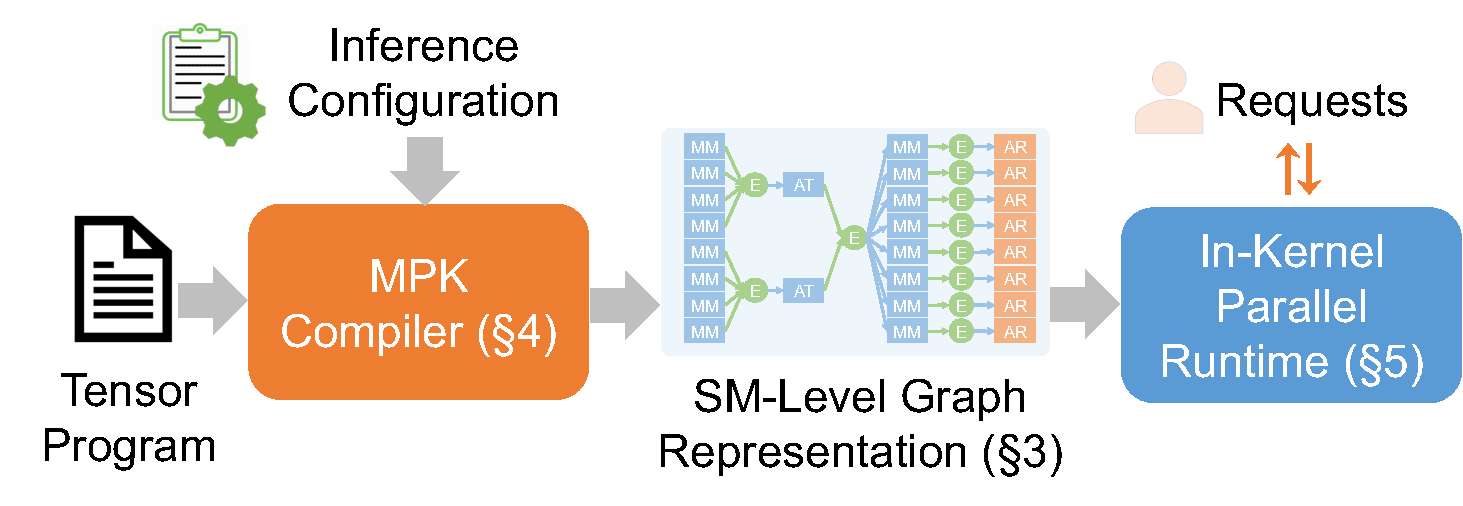
\includegraphics[width=\linewidth]{figs/overview_mpk.pdf}
 \vspace{\captionvspace}
 \caption{\sys 总览。}
 \vspace{\captionvspace}
 \label{fig:overview}
\end{figure}

\sys 的核心思想，是不再以整个 GPU，而是以单个流式多处理器（SM）为粒度表示计算与跨 GPU 通信。为此，\sys 引入了称为 \graph 的 {\em SM 级图表示}：图中的节点是运行在各个 SM 上的任务，边则刻画任务之间的细粒度依赖。这样的表示能够暴露更多并行性，并支持跨算子软件流水和细粒度 kernel 重叠等传统按算子逐核执行模型无法实现的优化。 \Cref{fig:overview} 展示了支撑这一思路的两个关键组件。

\paragraph{\Sys 编译器。}
\Sys 编译器以张量程序和推理配置为输入，自动将原始计算图转化为面向特定推理配置与 GPU 架构的高性能 SM 级 \graph。编译过程中，系统会执行事件融合、图规范化与图线性化等一系列优化，以降低同步开销并提升生成任务图的执行效率。此外，\Sys 还会基于已有的超级优化技术~\cite{wu2025mirage}，自动为每个任务生成高性能 CUDA 实现，从而保证 SM 级执行同样高效。

\paragraph{核内并行运行时。}
\Sys 通过一个完全嵌入在 mega-kernel 内部的并行运行时来执行 SM 级 \graph，从而在模型执行期间 {\em 不再需要任何额外的 kernel 启动}，并能以细粒度方式控制任务调度与执行。为实现这一点，运行时将 GPU 的 SM 划分为 {\em worker} 与 {\em scheduler} 两类角色。worker 维护本地任务队列，并按先进先出的顺序执行任务；scheduler 维护任务依赖，并在条件满足时将任务分发出去。整个运行时采用 {\em 事件驱动、完全异步} 的执行模型，以最大化 GPU 利用率。同时，\sys 结合即时启动与提前启动两种方式，形成 {\em 混合任务发射策略}，以在低开销和动态负载均衡之间取得平衡。

\paragraph{实验结果。}
我们将 \sys 实现为 PyTorch 的一个 kernel backend。用户只需修改少量代码，就可以把 PyTorch 程序编译成 \sys mega-kernel。我们在五个常见模型上，跨三代 NVIDIA GPU（A100、H100 和 B200）进行了评测。即便面对像 SGLang 和 vLLM 这类已经广泛部署并经过深度优化的按算子逐核执行系统，\sys 在单 GPU 与多 GPU 部署中仍然取得了 1.0--1.7$\times$ 的性能提升，并将 LLM 推理性能进一步推向硬件极限。
